\section{Gait generation}
\label{gaits}

Modular robot locomotion, with the large number of degrees of freedom that it usually involves requires highly
coordinated gaits in order to be efficient and effective. Several approaches to solve this coordination problem can be found in the literature, and have been already described on section \ref{state_art_controllers}.\\

Gait tables are a simple approach, but they are mainly used with a central control paradigm. They also lack flexibility, and their complexity increases with an increase in the number of degrees of freedom of the robot.\\

CPGs are very powerful controllers, but they are also very complex to model and implement, and highly redundant. These CPG mathematical models are useful for neurocomputing scientists to study biological CPGs and model neural circuits, as they can be tested either on simulations or on real robots, and therefore validated. In robotics, on the other hand, one is often more interesting in efficiency, in obtaining the best possible gaits using as less resources, computing power and power as possible.\\

Sinusoidal oscillators, as a simplification of CPGs, are the controller chosen for this work. The main reasons for choosing sinusoidal oscillators are:
\begin{itemize}
	\item Sinusoidal oscillators are simple and easy to model and implement. As the joint position follow a sinewave, they do not require a lot of computing power for their execution, so they can be embedded on a simple microcontroller.
	
	\item Once their paremeters are selected and set, they can oscillate independently from the rest of oscillators, making them more robust against communication problems. As each step of the joint position is generated by the oscillators, the modules can be synchronized less often, and a greater bandwidth is available for communicating other kind of messages.\\
\end{itemize}
                                                      

For modelling the sinusoidal oscillators, the following equation is used:
\begin{equation} \label{eq:sinusoidal_oscillator}
\varphi_i(t) = A_i \cdot \sin{\left( \frac{2\pi}{T} \cdot t + \Phi_i \right)} + O_i \qquad i \in \lbrace 1, ..., N \rbrace 1
\end{equation}\\


\begin{table}[h]
\centering
\begin{tabular}{|c||c|c|} \hline
Symbol & Description & Range \\ \hline \hline
$\varphi_i(t)$ & Position of the ith joint & [-90, 90] degrees \\ \hline
$A_i$ & Amplitude of the ith oscillator & [0, 90] degrees \\ \hline
$T$ & Period of the oscillator &  T > 0 seconds \\ \hline
$t$ & Elapsed time & t $\leq$ 0 seconds \\ \hline
$\Phi_i$ & Initial phase of ith oscillator & [0, 360] degrees \\ \hline
$O_i$ & Offset of ith oscillator & [-90, 90] degrees \\ \hline
$N$ & Number of modules in the robot & $N \geq 2$ \\ \hline
\end{tabular}
\caption{Parameters of the sinusoidal oscillator}
\end{table}

\newpage

The frequency of the oscillators does not affect the coordination, but the speed of the gait. The main parameter behind gait coordination is the phase of the oscillator, defined as:

\begin{equation} \label{eq:phase_of_time}
\phi(t) = \frac{2\pi}{T} \cdot t
\end{equation}\\

Which can be substituted in equation \ref{eq:sinusoidal_oscillator} to get the joint value of the ith oscillator as a function of the phase:

\begin{equation} \label{eq:sinusoidal_oscillator_phase}
\varphi_i(\phi) = A_i \cdot \sin{\left( \phi + \Phi_i \right)} + O_i \qquad i \in \lbrace 1, ..., N \rbrace 1
\end{equation}\\

As the modules are physically actuated by a hobby servo, with a mechanical restriction of 180 degrees, we have limited the oscillator joint values to  a range of [-90, 90] degrees, imposing the following restriction to the oscillator parameters:
\begin{equation} \label{eq:oscillator_restriction}
|O_i| + A_i \leq 90
\end{equation}

\newpage
Figure \ref{fig:oscillator_center_seq} helps to understand the physical meaning of the equation parameters. In this case, the amplitude is 45º and the offset is 0º, so the movement is centered around the 0º joint position. The minimum position reached by the joint is $ O - A = -45º$ and the maximum one is $O + A = 45º$, following a sinusoidal waveform as a function of time.\\

\begin{figure}[h]
		\centering
        \begin{subfigure}[b]{0.18\textwidth}
                \centering
                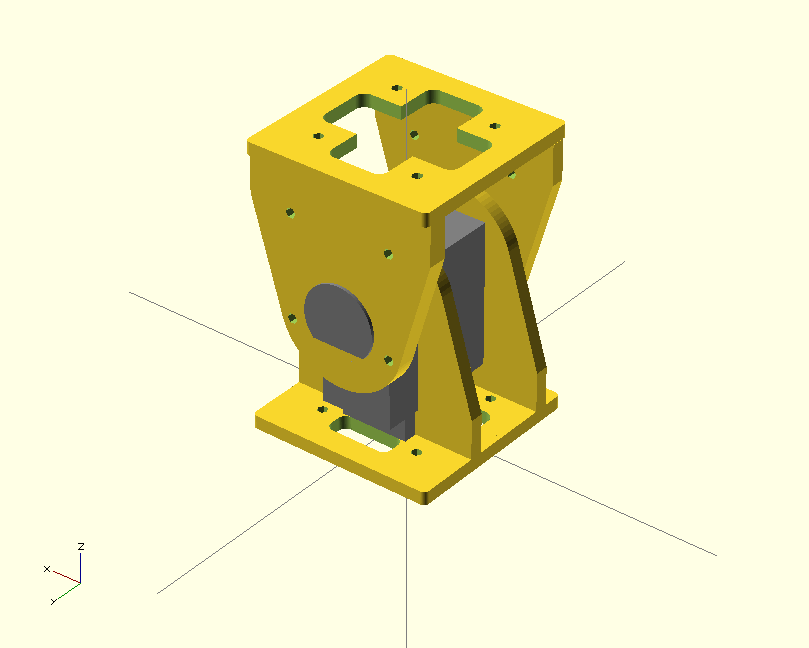
\includegraphics[width=\textwidth]{images/Gait_osc_center_90.png}
                 ~
                \label{fig:Gait_osc_center_90}
        \end{subfigure}
        ~
        \begin{subfigure}[b]{0.18\textwidth}
                \centering
                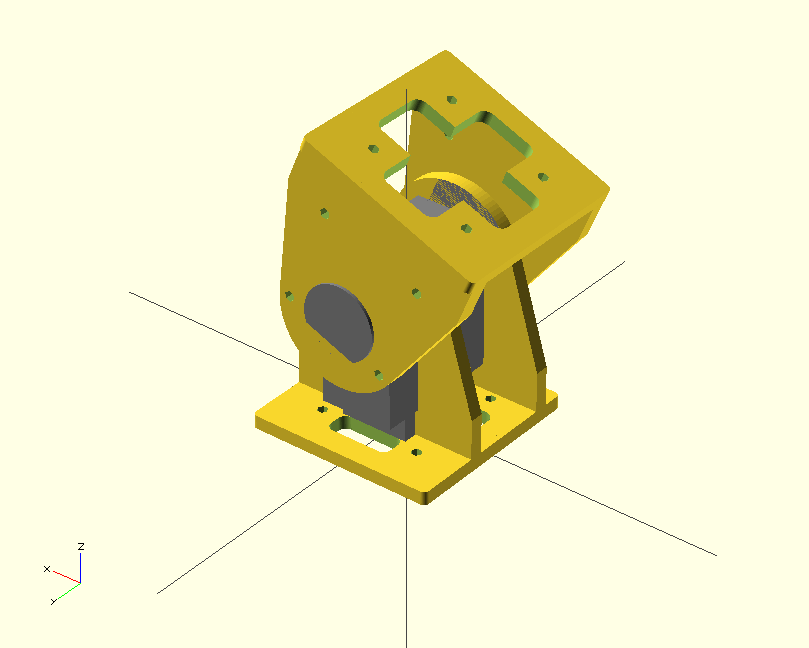
\includegraphics[width=\textwidth]{images/Gait_osc_center_112_5.png}
                 ~
                \label{fig:Gait_osc_center_112_5}
        \end{subfigure}
        ~
        \begin{subfigure}[b]{0.18\textwidth}
         	   \centering
                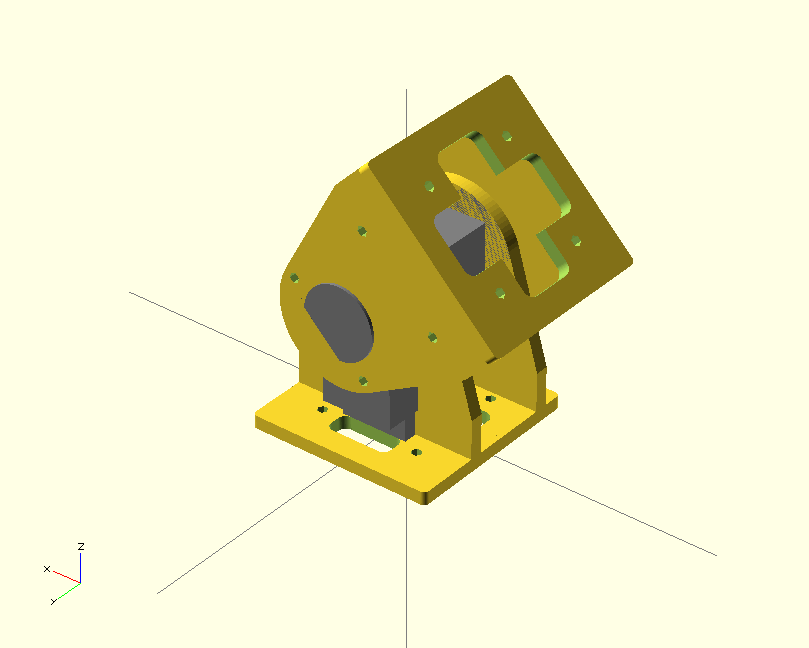
\includegraphics[width=\textwidth]{images/Gait_osc_center_135.png}
                ~
                \label{fig:Gait_osc_center_135}
        \end{subfigure}
        ~
        \begin{subfigure}[b]{0.18\textwidth}
         	   \centering
                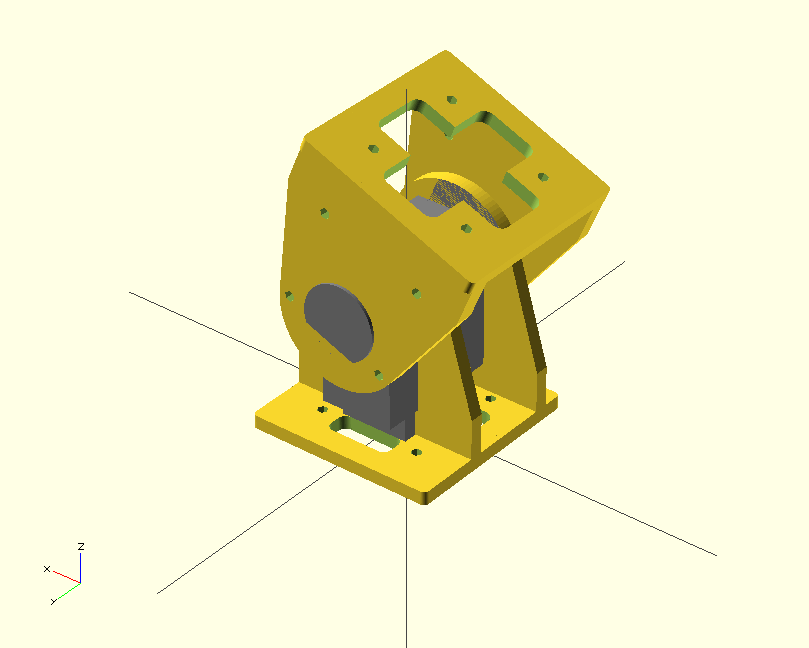
\includegraphics[width=\textwidth]{images/Gait_osc_center_112_5.png}
                ~
                \label{fig:Gait_osc_center_112_5-2}
        \end{subfigure}
        ~
        \begin{subfigure}[b]{0.18\textwidth}
         	   \centering
                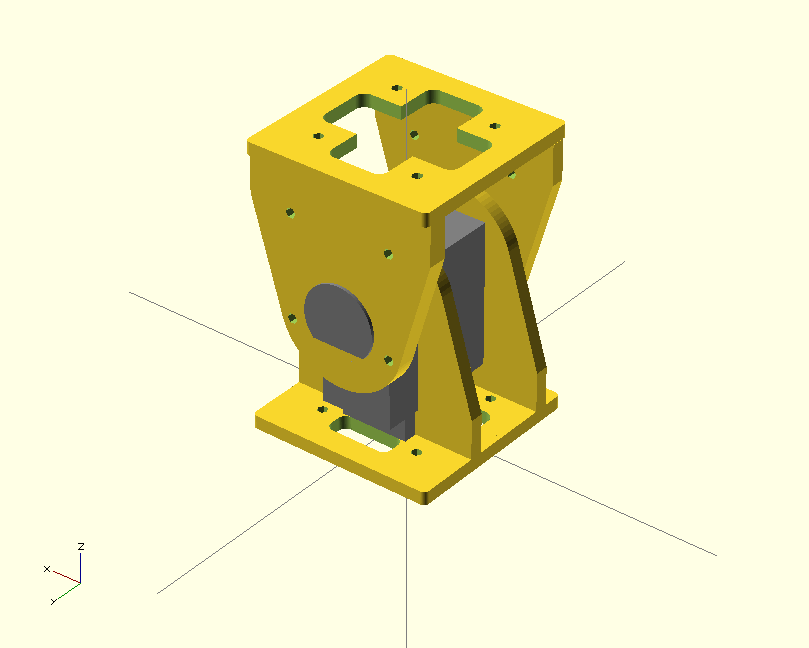
\includegraphics[width=\textwidth]{images/Gait_osc_center_90.png}
                 ~
                \label{fig:Gait_osc_center_90-2}
        \end{subfigure}
        ~
                \begin{subfigure}[b]{0.18\textwidth}
                \centering
                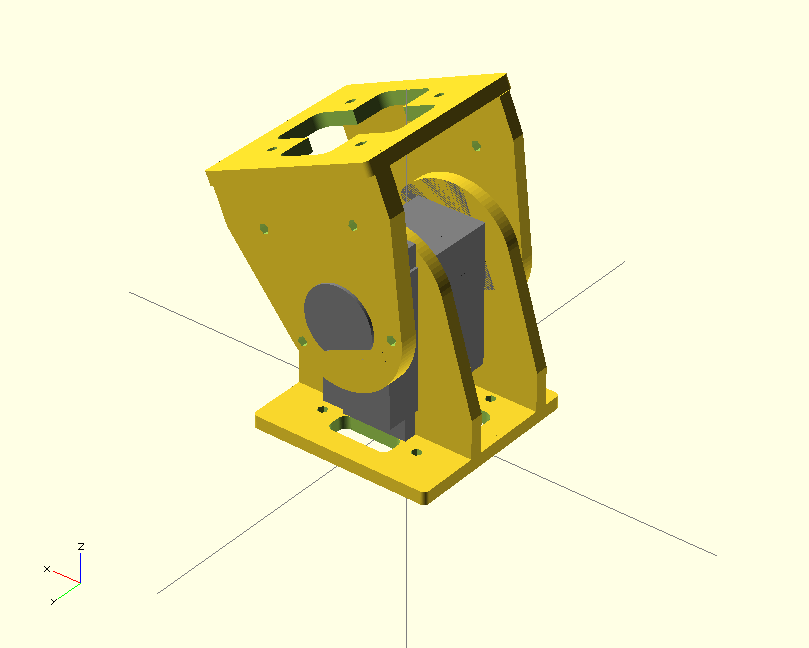
\includegraphics[width=\textwidth]{images/Gait_osc_center_62_5.png}
                ~
                \label{fig:Gait_osc_center_62_5-2}
        \end{subfigure}
        ~
        \begin{subfigure}[b]{0.18\textwidth}
                \centering
                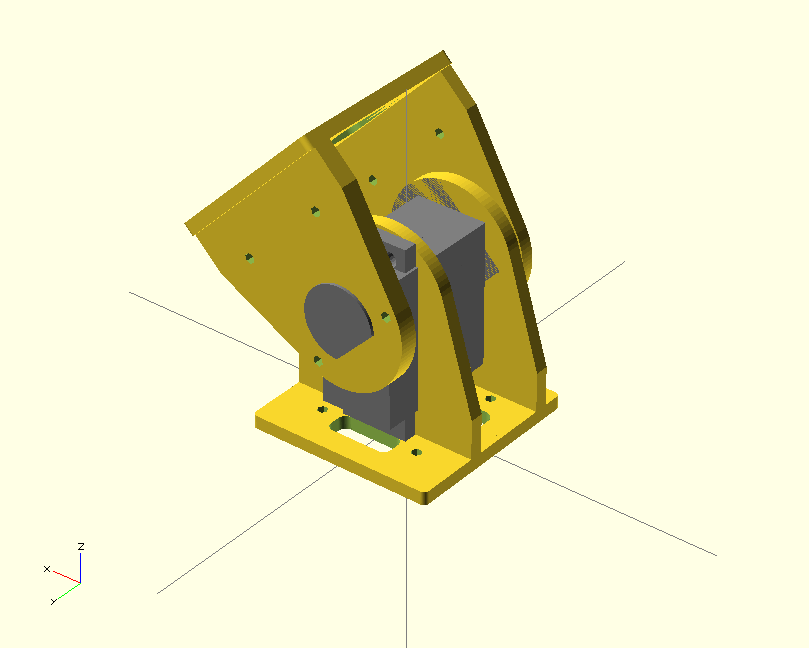
\includegraphics[width=\textwidth]{images/Gait_osc_center_45.png}
                 ~
                \label{fig:Gait_osc_center_45-2}
        \end{subfigure}
        ~
        \begin{subfigure}[b]{0.18\textwidth}
         	   \centering
                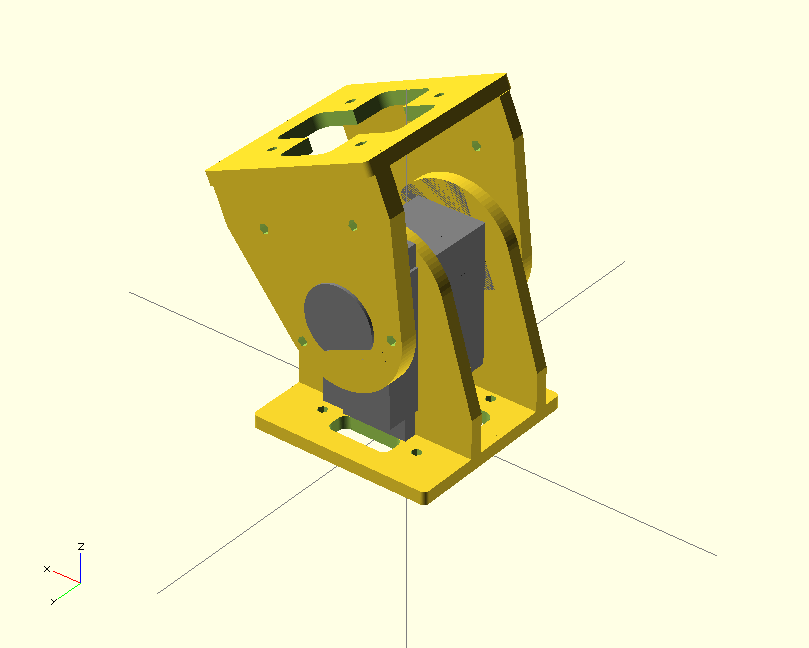
\includegraphics[width=\textwidth]{images/Gait_osc_center_62_5.png}
                 ~
                \label{fig:Gait_osc_center_62_5-3}
        \end{subfigure}
        ~
        \begin{subfigure}[b]{0.18\textwidth}
         	   \centering
                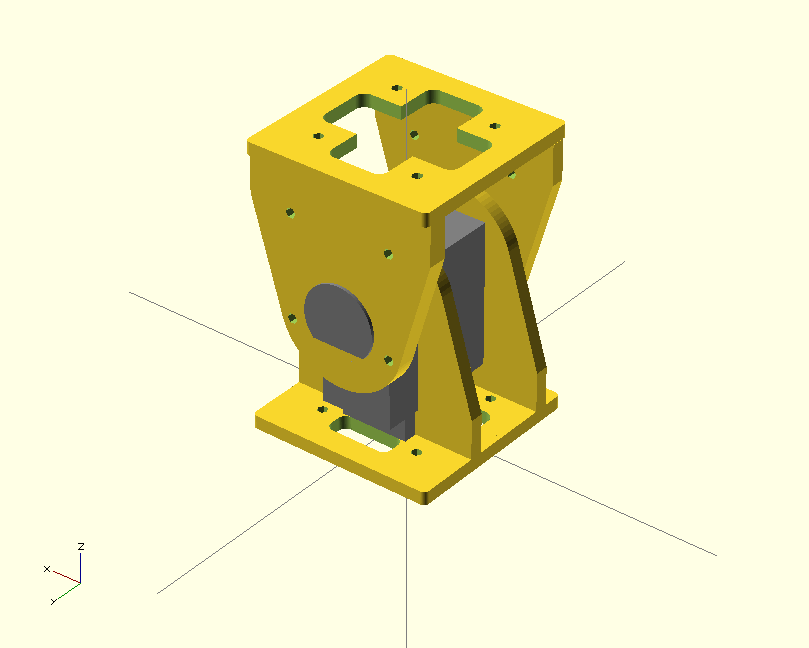
\includegraphics[width=\textwidth]{images/Gait_osc_center_90.png}
                 ~
                \label{fig:Gait_osc_center_90-3}
        \end{subfigure}
        \caption{Sequence of module oscillation for $A_i = 45º$, $O_i = 0º$}\label{fig:oscillator_center_seq}
\end{figure}

In figure \ref{fig:oscillator_offset_seq} the oscillator has the same amplitude as before, 45º, but the offset has been set to -45º. We can observe that in this case the movement is centered around -45º, with a minimum position at  $ O - A = -90º$ and a maximum one at $O + A = 0º$.\\

\begin{figure}[h]
		\centering
        \begin{subfigure}[b]{0.18\textwidth}
                \centering
                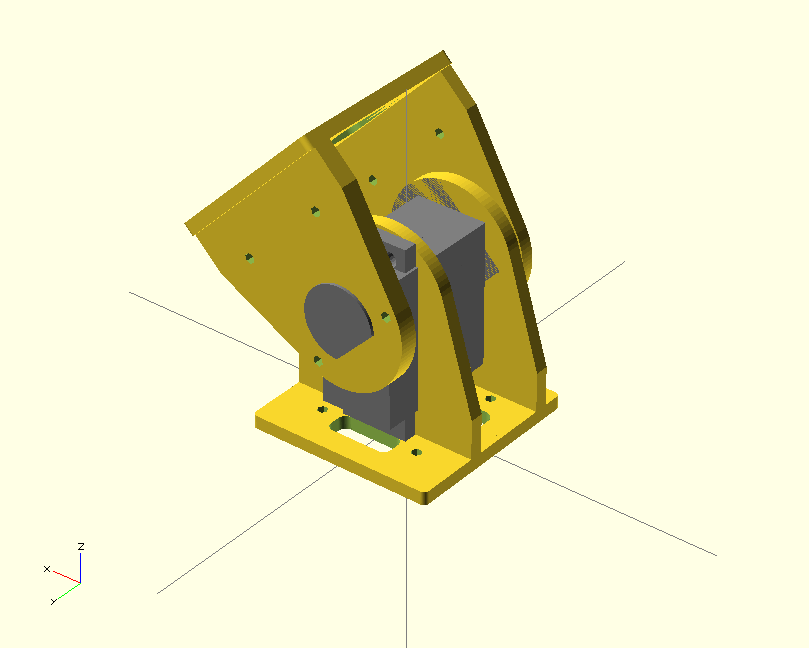
\includegraphics[width=\textwidth]{images/Gait_osc_offset_45.png}
                ~
                \label{fig:Gait_osc_offset_45}
        \end{subfigure}
        ~
        \begin{subfigure}[b]{0.18\textwidth}
                \centering
                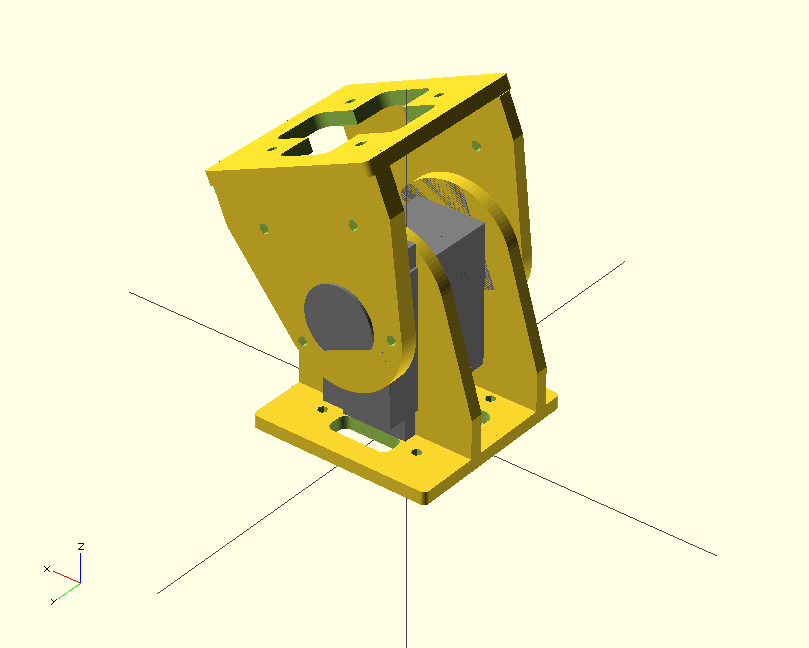
\includegraphics[width=\textwidth]{images/Gait_osc_offset_67_5.png}
                ~
                \label{fig:Gait_osc_offset_67_5}
        \end{subfigure}
        ~
        \begin{subfigure}[b]{0.18\textwidth}
         	   \centering
                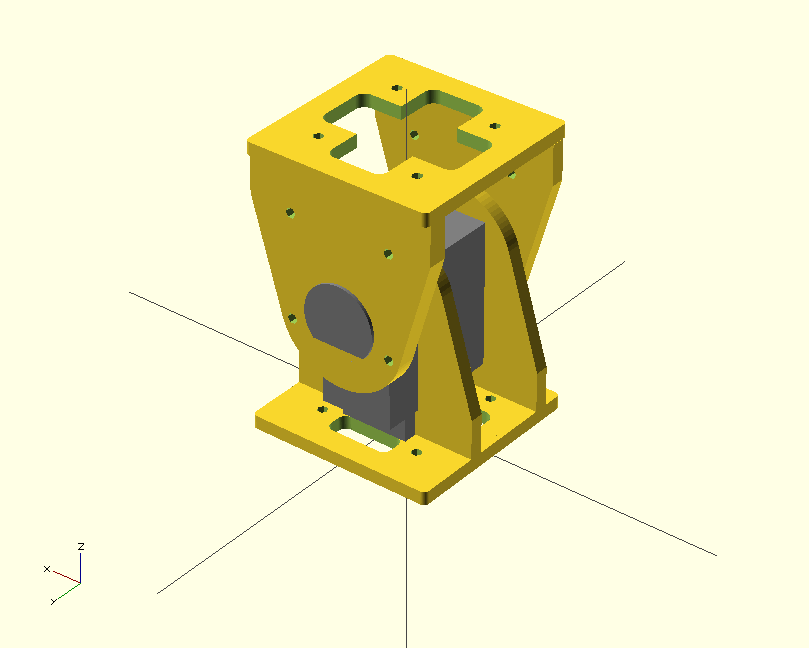
\includegraphics[width=\textwidth]{images/Gait_osc_offset_90.png}
                ~
                \label{fig:Gait_osc_offset_90}
        \end{subfigure}
        ~
        \begin{subfigure}[b]{0.18\textwidth}
         	   \centering
                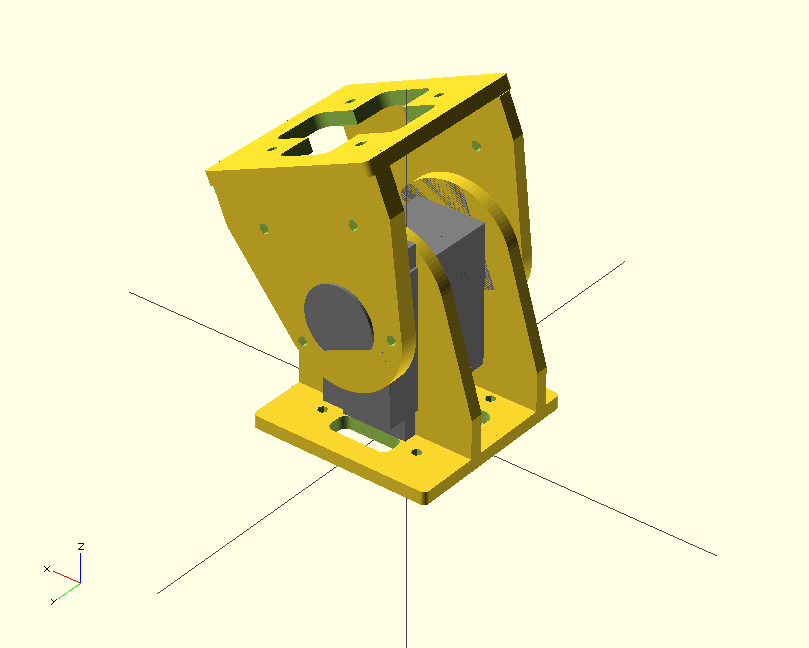
\includegraphics[width=\textwidth]{images/Gait_osc_offset_67_5.png}
                ~
                \label{fig:Gait_osc_offset_67_5-2}
        \end{subfigure}
        ~
        \begin{subfigure}[b]{0.18\textwidth}
         	   \centering
                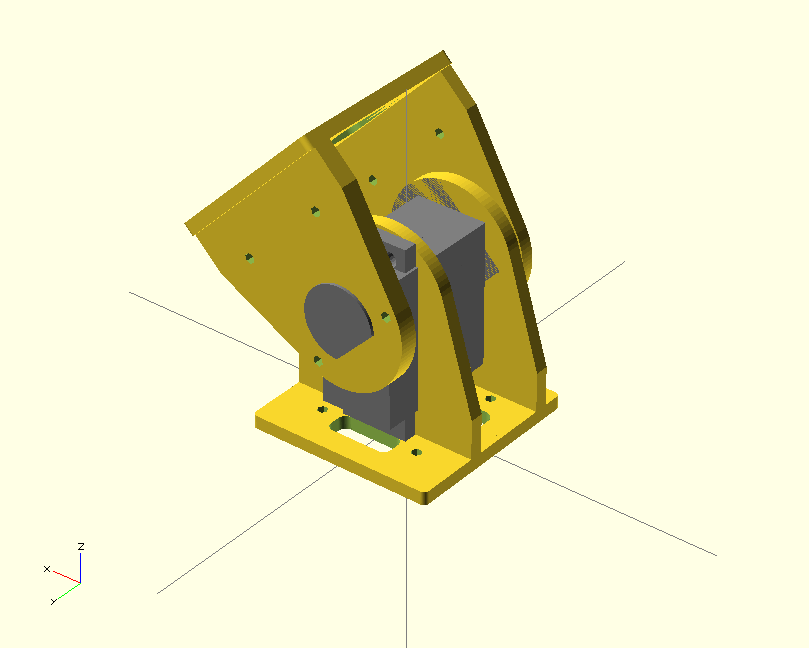
\includegraphics[width=\textwidth]{images/Gait_osc_offset_45.png}
                ~
                \label{fig:Gait_osc_offset_45-2}
        \end{subfigure}
        ~
                \begin{subfigure}[b]{0.18\textwidth}
                \centering
                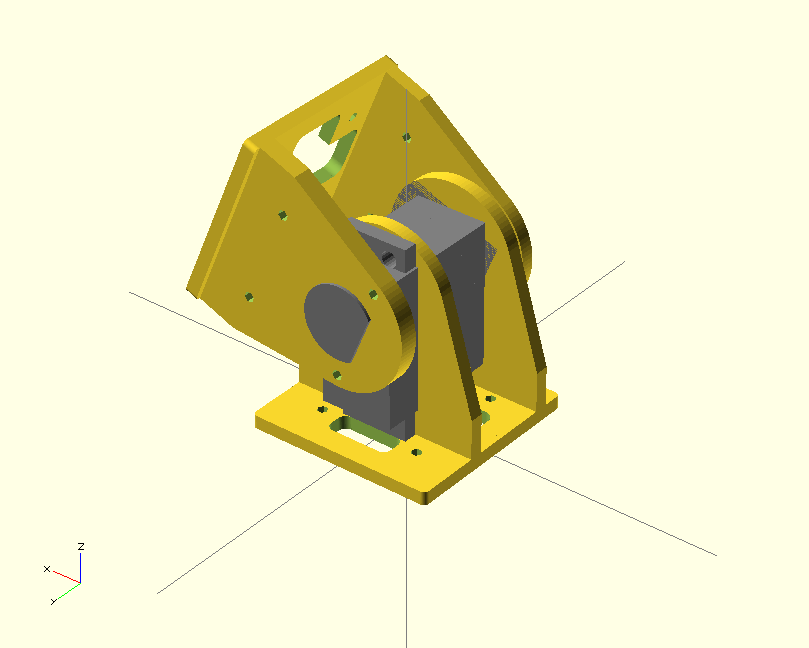
\includegraphics[width=\textwidth]{images/Gait_osc_offset_22_5.png}
                 ~
                \label{fig:Gait_osc_offset_22_5-2}
        \end{subfigure}
        ~
        \begin{subfigure}[b]{0.18\textwidth}
                \centering
                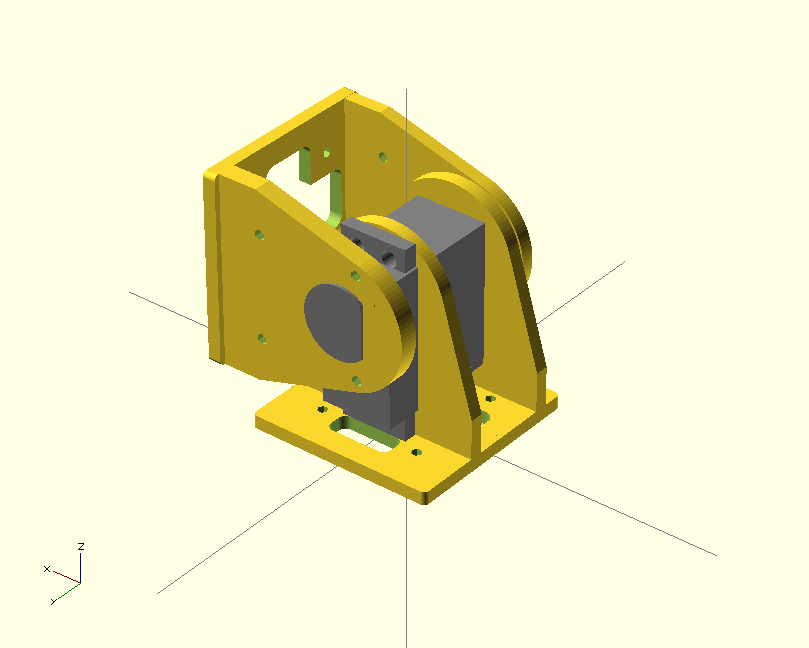
\includegraphics[width=\textwidth]{images/Gait_osc_offset_0.png}
                 ~
                \label{fig:Gait_osc_offset_0-2}
        \end{subfigure}
        ~
        \begin{subfigure}[b]{0.18\textwidth}
         	   \centering
                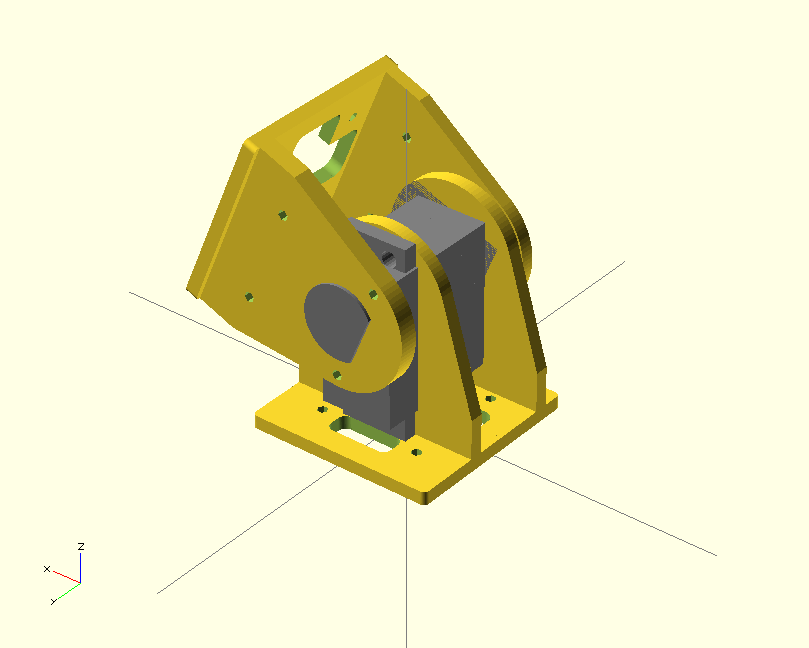
\includegraphics[width=\textwidth]{images/Gait_osc_offset_22_5.png}
                 ~
                \label{fig:Gait_osc_offset_22_5-3}
        \end{subfigure}
        ~
        \begin{subfigure}[b]{0.18\textwidth}
         	   \centering
                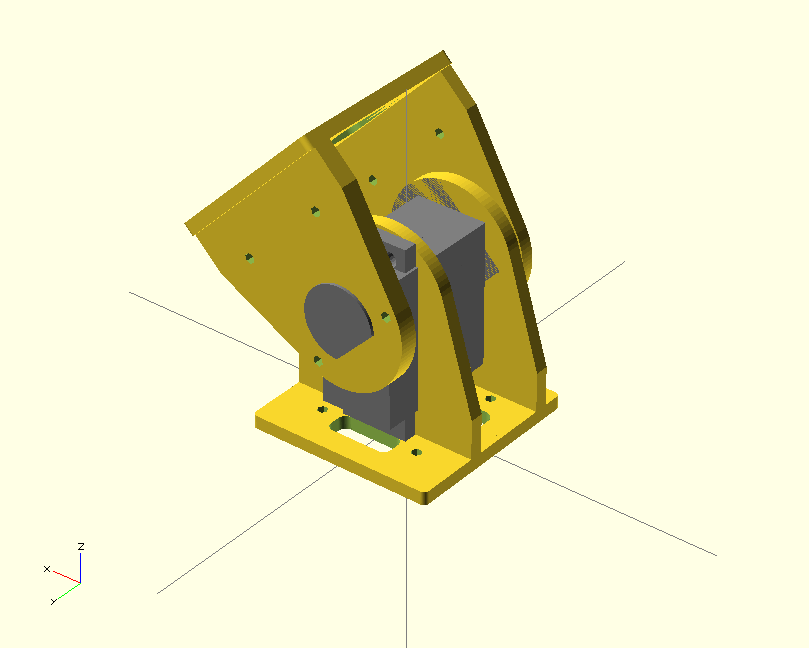
\includegraphics[width=\textwidth]{images/Gait_osc_offset_45.png}
                 ~
                \label{fig:Gait_osc_offset_45-3}
        \end{subfigure}
        \caption{Sequence of module oscillation for $A_i = 45º$, $O_i = -45º$}\label{fig:oscillator_offset_seq}
\end{figure}

